
\documentclass[a4paper,12pt]{article}

\usepackage{cmap}					
\usepackage[T2A]{fontenc}
\usepackage[utf8]{inputenc}
\usepackage[english,russian]{babel}
\usepackage{hyperref}
\usepackage{graphicx}

\hypersetup{
    colorlinks=true,
    linkcolor=blue,
    filecolor=magenta,      
    urlcolor=cyan,
}

\usepackage{amsmath,amsfonts,amssymb,mathtools}
\usepackage{icomma}

\usepackage{euscript}
\usepackage{mathrsfs}
\usepackage{graphicx}
\usepackage{eso-pic}
\usepackage{tikzlings-owls}


\newcommand*{\hm}[1]{#1\nobreak\discretionary{}%
{\hbox{$\mathsurround=0pt #1$}}{}}
\graphicspath{ {images/} }


\title{Дифференциальное уравнение движения маятника}

\author{Раков Николай, Булкина Милена\\M3236}
\date{\today}

\begin{document}

\maketitle
\tableofcontents{}
\clearpage

\section{Математический маятник}
\begin{tikzpicture}
\owl[scale=0.5]
\thing[beret,scale=0.6,yshift=-0.35cm,xshift=0.1cm]
\thing[handbag,scale=0.6,yshift=-0.3cm,xshift=0.1cm]
\thing[wine,scale=0.6,yshift=-0.0cm,xshift=-0.5cm]
\end{tikzpicture}


Математический маятник представляет собой идеальную модель, в которой материальная точка массой m подвешена на невесомой и нерастяжимой струне.
Когда маятник смещен из своего исходного положения в начальный угол и отпущен, периодическое движение свободно качается взад-вперед.


\section{Дифференциальное уравнение движения}

Запишем второй закон Ньютона для вращательного движения:
\begin{equation}\label{newton}
    \tau = I\alpha = I\frac{d^2\theta}{dt^2}
\end{equation}
где $\tau$ - момент силы, 
I - момент инерции тела относительно оси вращения,
$\alpha$ - угловое ускорение.
\\В нашем случае момент силы определяется проекцией силы тяжести на тангенциальное направление, т.е.
\begin{equation}
    \tau = -mgL\sin{\theta}
\end{equation}
Момент инерции маятника выражается формулой:
\begin{equation}
    I = mL^2
\end{equation}
Тогда уравнение \eqref{newton} принимает вид:
\begin{equation}\label{pre-final}
    -mgL\sin\theta = mL^2\frac{d^2\theta}{dt^2}
\end{equation}

\begin{equation}\label{final}
    \frac{d^2\theta}{dt^2} = -\frac{g}{L}sin\theta
\end{equation}

\section{Точное решение}

Для корректного описания колебательной системы нужно решать уравнение.


\begin{equation}
\frac{d^2\theta}{dt^2} + \frac{g}{L}sin\theta = 0
\end{equation}
Мы будем рассматривать колебания при начальных условиях:
\begin{equation}\label{nachal'noe}
    \theta(0) = \theta_0\;\; \left(\frac{d\theta}{dt}\right)(t = 0) = 0
\end{equation}
где $\theta_0$ - амплитуда колебаний
\\Понизим порядок данного уравнения умножив на интегрирующий множитель $\dfrac{d\theta}{dt}$. Получим уравнение:
\begin{equation}
    \frac{d^2\theta}{dt^2}\frac{d\theta}{dt} + \frac{g}{L}sin\theta\frac{d\theta}{dt} = 0
\end{equation}
\begin{equation}
    \frac{d}{dt}\left(\frac{1}{2}\left(\frac{d\theta}{dt}\right)^2 - \frac{g}{L}cos\theta\right) = 0
\end{equation}
Интегрируем и получаем уравнение 1-го порядка:
\begin{equation}
    \left(\frac{d\theta}{dt}\right)^2 - 2\frac{g}{L}cos\theta = C
\end{equation}
Находим C:
\begin{equation}
C = 2\frac{g}{L}cos\theta_0
\end{equation}
Получаем уравнение:
\begin{equation}
    \left(\frac{d\theta}{dt}\right)^2 - 2\frac{g}{L}cos\left(\theta - \theta_0\right) = 0
\end{equation}
Применим тригонометрическую формулу двойного угла:
\begin{equation}
    \cos{\theta} = 1 - 2\sin^2{\dfrac{\theta}{2}}
\end{equation}
в следствии чего получим следующее дифференциальное уравнение
\begin{equation}
    \frac{d\theta}{dt} - 2\sqrt{\frac{g}{L}}\sqrt{sin^2\frac{\theta_0}{2} - sin^2\frac{\theta}{2}} = 0
\end{equation}
\begin{equation}\label{dtheta:dt}
    \left(\frac{d\theta}{dt}\right)^2 = 
    \frac{4g}{L}\left(sin^2\frac{\theta_0}{2} - sin^2\frac{\theta}{2}\right)
\end{equation}
Введем обозначения:
\begin{equation}
    y = sin{\frac{\theta}{2}} \;\text{и}\; k = sin^2{\frac{\theta_0}{2}}
\end{equation}
Исходя из уравнения \eqref{nachal'noe} получаем:
\begin{equation}
    y(0) = \sqrt{k}
\end{equation}
Выразим $\dfrac{dy}{dt}$:
\begin{equation}
    \dfrac{dy}{dt} = \dfrac{dy}{d\theta}\dfrac{d\theta}{dt} =
    \dfrac{1}{2}\cos{\dfrac{\theta}{2}}\dfrac{d\theta}{dt}
\end{equation}
\begin{equation}
    \left(\dfrac{dy}{dt}\right)^2 = 
    \dfrac{1}{4}\cos^2\left({\dfrac{\theta}{2}}\right)\left(\dfrac{d\theta}{dt}\right)^2
\end{equation}
Выразим $\dfrac{d\theta}{dt}$:
\begin{equation}
    \left(\dfrac{d\theta}{dt}\right)^2 = 
    \frac{4}{\cos^{2}\left({\frac{\theta}{2}}\right)}\left(\dfrac{dy}{dt}\right)^2 =
    \frac{4}{1-y^2}\left(\dfrac{dy}{dt}\right)^2
\end{equation}
Из \eqref{dtheta:dt}:
\begin{equation}
    \frac{4}{1-y^2}\left(\dfrac{dy}{dt}\right)^2 = 
    \frac{4g}{L}\left(k - y^2\right)
\end{equation}
Из чего получим:
\begin{equation}\label{dy/dt1}
    \left(\dfrac{dy}{dt}\right)^{2} =
    \dfrac{g}{L}k\left(1 - y^2\right)\left(1 - \dfrac{y^2}{k}\right)
\end{equation}
Введем обозначения:
\begin{equation}
    \tau = t\sqrt{\frac{g}{L}} \;\text{и}\; 
    z = \frac{y}{\sqrt{k}}
\end{equation}
Из \eqref{dy/dt1} получаем:
\begin{equation}\label{dy/dt2}
    \left(\frac{dz}{d\tau}\right)^2 = 
    (1 - z^2)(1 - zk^2)
\end{equation}
\begin{equation}
    z(0) = 1  \;\; \left(\frac{dz}{d\tau}\right)(\tau = 0) = 0
\end{equation}
Выразим d$\tau$ из \eqref{dy/dt2}:
\begin{equation}
    d\tau = \pm\dfrac{dz}{\sqrt{(1-z^2)(1-kz^2)}}
\end{equation}
Интегрируем по отрезку [1, z]
\begin{equation}\label{beta}
    \tau =
    - \int_{1}^{z}\dfrac{d\beta}{\sqrt{(1-\beta^2)(1-k\beta^2)}}
\end{equation}
Уравнение \eqref{beta} также может быть представлено в виде:
\begin{equation}\label{tau}
    \tau = \int_{0}^{1}\dfrac{d\beta}{\sqrt{(1-\beta^2)(1-k\beta^2)}} -
    \int_{0}^{z}\dfrac{d\beta}{\sqrt{(1-\beta^2)(1-k\beta^2)}}
\end{equation}
Интеграл
\begin{equation}
    F\left(\gamma; k\right) = \int_{0}^{sin{\gamma}}\dfrac{dx}{\sqrt{(1-x^2)(1-k^2x^2)}}
\end{equation}
называется эллиптическим инегралом первого рода. А интеграл
\begin{equation}
    K(k) = \int_{0}^{1}\dfrac{dx}{\sqrt{(1-x^2)(1-k^2x^2)}}
\end{equation}
называется полным эллиптическим интегралом первого рода.
\\Также эллиптический синус задаётся как:
\begin{equation}
    sn(u; k) = \sin{\gamma}
\end{equation}
Уравнение \eqref{tau}  может быть записано так:
\begin{equation}
    \tau = K(k) - F\left(\arcsin{z};\; \sqrt{k}\right)
\end{equation}
\begin{equation}
    F\left(\arcsin{z};\; \sqrt{k}\right) = K(k) - \tau
\end{equation}
Можем выразить с помощью эллиптического синуса:
\begin{equation}
    \dfrac{\sin{\frac{\theta}{2}}}{\sin{\frac{\theta_0}{2}}} =
    sn\left(K\left(\sin^2{\dfrac{\theta_0}{2}}\right) -
    \sqrt{\frac{g}{L}}t;\; \sin^2{\frac{\theta_0}{2}}\right)
\end{equation}
Выразим $\theta$ как функцию от t:
\begin{equation}
    \theta(t) = 2\arcsin{\left[
    sin{\dfrac{\theta_0}{2}}sn\left(K\left(\sin^2{\dfrac{\theta_0}{2}}\right) -
    \sqrt{\frac{g}{L}}t;\; \sin^2{\frac{\theta_0}{2}}\right)\right]}
\end{equation}

\section{Приближенное решение}

\subsection{Малые колебания}

В случае малых колебаний полагают, что  $\sin{\alpha} \approx  \alpha$.  В результате возникает линейное дифференциальное уравнение:
\begin{equation}
\frac{d^2\theta}{dt^2} = -\frac{g}{L}\theta
\end{equation}

Составим характеристическое уравнение
\begin{equation}
\lambda^2 + \frac{g}{L} = 0
\end{equation}

Получим два комплексно-сопряженных корня
\begin{equation}
\lambda_{1,2} = \pm i \sqrt{\frac{g}{L}}
\end{equation}

Запишем решение уравнения
\begin{equation}
\theta(t) = \theta_0 \cos{\sqrt{\frac{g}{L}} t} + \theta_1 \sin{\sqrt{\frac{g}{L}} t}
\end{equation}

Получаем период малых колебаний
\begin{equation}
\theta(t) = \theta_0\cos{\left(\sqrt{\frac{g}{L}}t+\delta\right)}
\end{equation}
где $\theta_0$ - это амплитуда колебаний 
а $\delta$ - начальная фаза колебаний

\subsection{Разложение в ряд Фурье}
Разложим полученную выше $\theta(t)$ в ряд Фурье:
\begin{equation}
     \theta (t)=8\sum _{n\geq 1{\text{ odd}}}{\frac {(-1)^{\left\lfloor {n/2}\right\rfloor }}{n}}{\frac {q^{n/2}}{1+q^{n}}}\cos(n\omega t)
\end{equation}
Где q - эллиптический ном $q=\exp(-\pi K'/K)$ и $\omega$ - угловая частота.
\\Введем обозначение:
\begin{equation}
    \epsilon ={\frac {1-{\sqrt {\cos {\frac {\theta _{0}}{2}}}}}{2+2{\sqrt {\cos {\frac {\theta _{0}}{2}}}}}}
\end{equation}
тогда можем представить q таким образом:
\begin{equation}
    {\displaystyle q=\epsilon +2\epsilon ^{5}+15\epsilon ^{9}+150\epsilon ^{13}+1707\epsilon ^{17}+20910\epsilon ^{21}+\cdots }
\end{equation}

\subsection{Использование численных методов Рунге-Кутты}
Для подсчета можно также использовать метод Рунге-Кутты четвертого порядка для достаточно точных вычислений.
\\Так, если у нас есть $y' = f(x, y),\quad y(x_{0})=  y_{0}$, можем вычислить приближенное значение в следующих точках $ y_{n+1} = y_n + {\frac{h}{6}}(k_1 + 2k_2 + 2k_3 + k_4)$
\\h - это величина сетки по x, тогда ошибка на одном шаге будет $\mathcal{O}(h^5)$

\section{Моделирование}

\subsection{Анализ методов вычисления}

\begin{figure}[!htb]
\minipage{0.50\textwidth}
  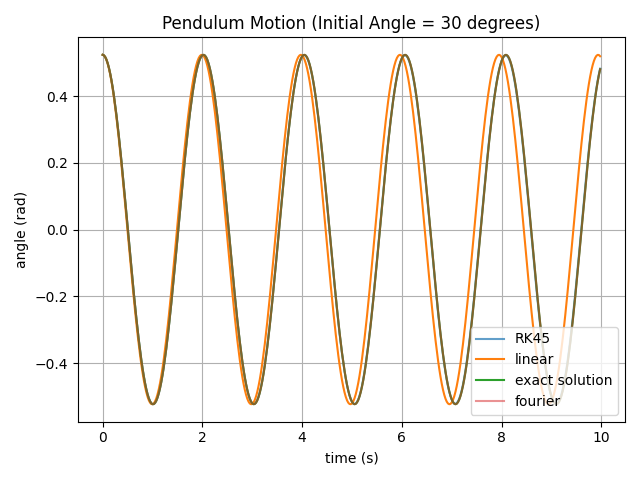
\includegraphics[width=\linewidth]{30.png}\label{30}
\endminipage\hfill
\minipage{0.50\textwidth}
  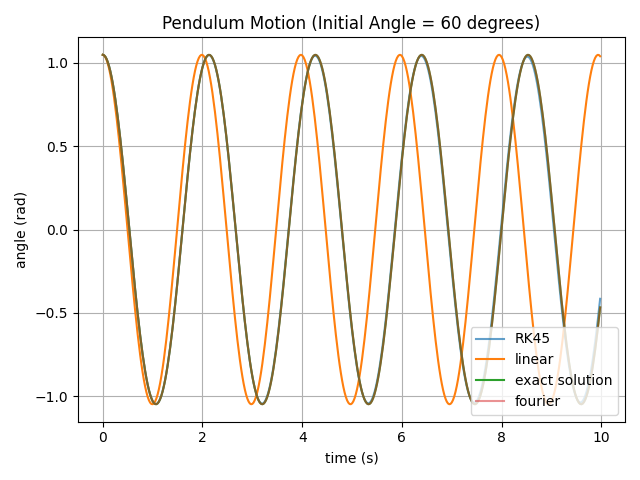
\includegraphics[width=\linewidth]{60.png}\label{60}
\endminipage\hfill
\end{figure}

\begin{figure}[!htb]
\minipage{0.50\textwidth}
  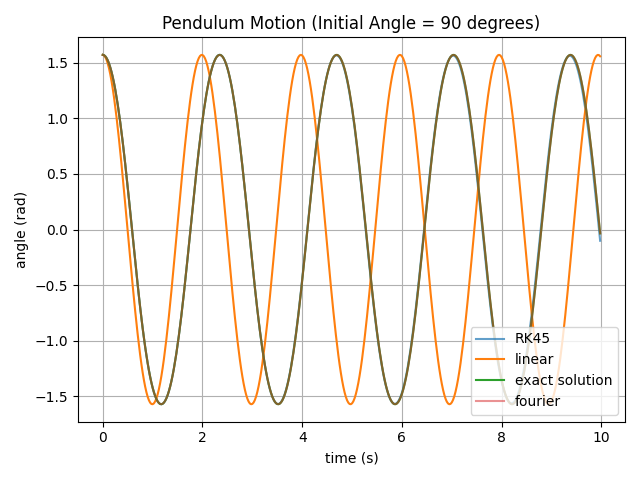
\includegraphics[width=\linewidth]{90.png}\label{90}
\endminipage\hfill
\minipage{0.50\textwidth}
  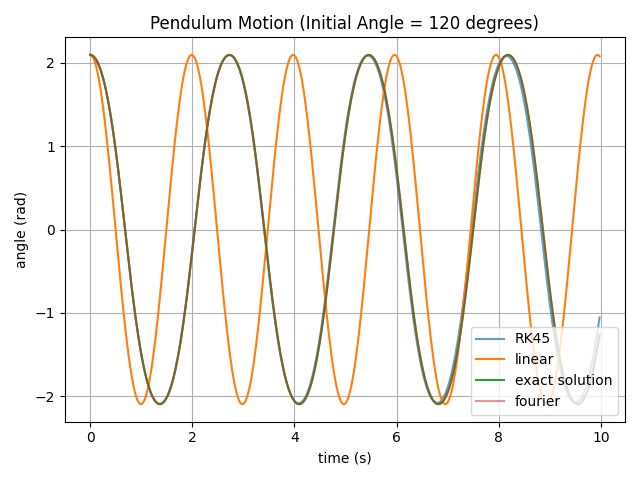
\includegraphics[width=\linewidth]{120.png}\label{120}
\endminipage\hfill
\end{figure}

\begin{figure}[!htb]
    \centering
    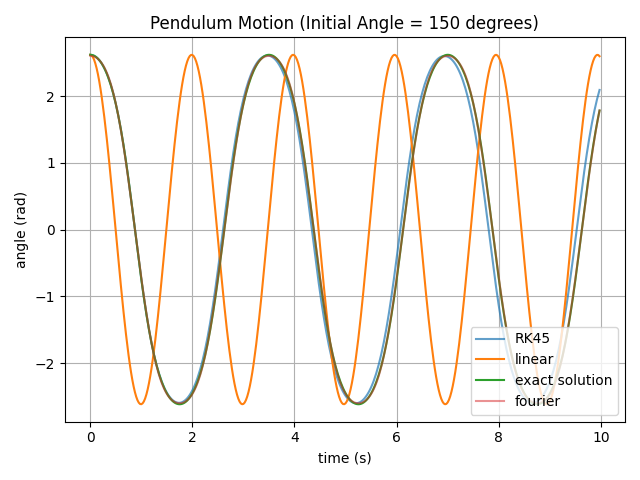
\includegraphics[width=70mm]{150.png}
\end{figure}
По графикам можем предположить, что разложение в ряд Фурье является более точным, чем метод Рунге-Кутта. Линейное же решение дает существенные отклоения уже при 30 градусах.

\subsection{Особенности реализации}

Поскольку движение маятника является периодическим, то имеет смысл просчитать значения только один раз и далее использовать только готовые значения, не пересчитывая каждый раз, это открывает возможность для ещё одной оптимизации, несколько маятников с одинаковой моделью движения могут разделять просчитанные значения функции.

Для вычислений был выбран метод Рунге-Кутты четвёртого порядка, как простой и вполне подходящий для данной задачи.

Теперь самое интересное! Представьте, что Вы - котик, путешествующий во сне по раскачивающимся клубкам мироздания и чем больше клубков Вы соберете, тем мощнее будут Ваши лапищи.

Игровая механика схожа с angry birds. Выбираем направление полета котика, силу прыжка, целью же является приземление кота на маятник. Важно, что прыгать на один и тот же маятник нельзя. Удачи!


\end{document}